\chapter{IRK: Eguzki-sistema.}


\section{Sarrera.}
  

Atal honetan, eguzki-sistemaren ekuazio diferentzialei Kepler-en fluxuan oinarritutako aldagai aldaketa aplikatzea proposatuko dugu. Aurreko ataletan, (\ref{chap:IRK-PF}~atala) puntu-finkoaren iterazioan  eta (\ref{chap:IRK-NEW}~atala) Newton sinplifikatuaren iterazioan oinarritutako IRK  inplementazioak garatu ditugu; eguzki-sistemaren problemaren integraziorako, bi inplementazioen artean,  puntu-finkoarena eraginkorragoa dela baieztatu dugu. Hortaz, puntu-finkoaren iterazioan oinarritutako IRK inplementazioa erabiliko dugu eta  ekuazio diferentzialei aplikatutako aldagai aldaketaren bidez, integrazio eraginkorra lortzea espero dugu.  

Aldagai aldaketaren bidez aplikatzen dugun integrazio metodoa, sinplektikoa eta simetrikoa da: neurri batean, Splitting metodoen baliokidea. Aldagai berriekiko ekuazio diferentzialak, magnitude txikiko balioak hartzen dituzte eta honek, hiru abantaila eragingo ditu. Lehenik, eguzki-sistemaren problemaren trunkatze errore nagusiena ezabatzen dugunez, urratsa luzera handiak erabili ahal izango ditugu. Bigarrenik, batura konpensatuaren konputazioan, informazio gutxiago galduko dugu. Jacobiarraren balioa txikia denez, puntu-finkoaren iterazioek konbergentzia azkarra izango dute. 

Lehenengo, Kepler-en fluxuaren inplementazioa azalduko dugu. Bigarrenik, aldagai aldaketa definitu eta metodoa integratzeko zehaztapenak emango ditugu. Hirugarrenik, eguzki-sistemaren problemaren zenbakizko integrazioak egingo ditugu: inplementazio honen eta doitasun altuko beste metodo sinplektikoen eraginkortasunak, alderatuko ditugu.         

 

\section{Kepler-en fluxua.}
   
Kepler problema, bi gorputzen problemaren kasu partikularra da eta  honako Hamiltondarra dagokio,
\begin{equation}
H(q,p)=\frac{p^2}{2m}-\frac{\mu}{\|q\|},
\end{equation}
non $m$ eta $\mu$ konstanteen balioak, formulazioaren araberakoak diren.

Koordenatu sistema $q=q_2-q_1$ duen formulazioa aukeratzen badugu, konstanteen balioak hauek dira,  
\begin{equation*}
m=(1/m_1+1/m_2)^{-1},\ \ \mu=Gm_1m_2,
\end{equation*} 

eta ekuazio diferentzialak era honetan definitzen dira,
\begin{equation}
\label{eq:kode}
\dot{q}=p, \ \ \dot{p}= - \frac{k \ q}{\|q\|^3} ,
\end{equation}
non $k= \mu / m$ eta  $q,p \in \mathbb{R}^3$.

Kepler problemaren soluzio zehatza kalkula daiteke: une bateko kokapen eta abiadurak emanik, denbora tarte bat ($\Delta t$) igarotakoan (positiboa ala negatiboa), kokapen eta abiadura zehatzak konputatu daitezke. Eguzki-sistemaren integrazio metodoentzat, Kepler problema doitasun handian eta era eraginkorrean kalkulatzea, funtsezkoa da. Kepler problemaren erreferentziazko inplementazioak, Danby \cite{Danby1992} eta J.Wisdom-renak  \cite{Wisdom2015} ditugu. 

Kepler-en fluxua, era honetan kalkulatzen da. Lehenik, koordenatu cartesiarretatik ($q,p\in \mathbb{R}^3$), koordenatu eliptikoetara $(a,e,i,\Omega,E)$, itzulpena egingo dugu. Koordenatu eliptikoetan, $E$ (\emph{eccentric anomaly}) aldagaia izan ezik, beste aldagaiak konstante mantentzen dira: beraz $E_0$ balioa emanda, $\Delta t$ denbora tartea aurrera egin eta $E_1$ balioa berria kalkulatuko dugu. Azkenik, koordenatu eliptikoetatik koordenatu cartesiarretara itzulpena eginez, kokapen eta abiadura berriak eskuratuko ditugu. 

\begin{equation*}
(q_0,v_0) \in \mathbb{R}^6 \ \ \ \longrightarrow \ \ \  (a,e,i,\Omega,E_0) \in \mathbb{R}^6 
\end{equation*}
\begin{equation*}
\quad \quad \quad \quad \quad \quad \quad \quad \downarrow \Delta t
\end{equation*}
\begin{equation*}
(q_1,v_1) \in \mathbb{R}^6 \ \ \ \longleftarrow \ \ \  (a,e,i,\Omega,E_1) \in \mathbb{R}^6 
\end{equation*}

Gorputz baten orbita Kepleriarra hiru motakoa izan daiteke: $H(q_0,p_0)<0$ denean orbita eliptikoa da, $H(q_0,p_0)>0$ orbita hiperbolikoa eta $H(q_0,p_0)=0$ orbita  paraboliko. Kepler fluxuaren C inplementazioa, orbita eliptikoetarako garatu dugu eta zehaztasunak, \ref{erans:B1} eranskinean eman ditugu. (\ref{eq:kode}) problemari dagokion fluxua, era honetan defini daiteke,
\begin{align*}
\varphi_{\Delta t}^k:&  \quad \mathbb{R}^{6} \quad  \longrightarrow \quad \mathbb{R}^6,  \\
&  \quad y_0 \ \  \rightsquigarrow \ \ y_1. 
\end{align*} 
non $y=(q,v) \in \mathbb{R}^6$  den.


\section{Inplementazioa.}


\subsection*{Aldagai aldaketa.}
Era honetako Hamiltondar sistemak $H: \mathbb{R} \times \mathbb{R}^{2d} \longrightarrow \mathbb{R}$, 
\begin{align}
\begin{split}
&H(q,p,t)=H_K(q,p)+H_I(q,p,t)
\end{split}
\end{align} 
hartuko ditugu kontutan: $H_K$  Kepleriarrari dagokion Hamiltondarraren  eta $H_I$ perturbazioei dagokion Hamiltondarraren aldeak dira.  

Notazio hau finkatuko dugu: $(q,p) \in \mathbb{R}^{2d}$ jatorrizko aldagaientzako eta $(Q,P) \in \mathbb{R}^{2d}$ aldagai berrientzako.
Kepler fluxua kalkulatzen duen funtzioa $\varphi_{\Delta t}^K(q,p) \in \mathbb{R}^{2d}$ bada, era honetan definituko dugu aldagaia aldaketa,
\begin{align}
\label{eq:aldak}
&(q,p)=\varphi_{\Delta t}^K(Q,P) \quad \text{edo} \quad \ (Q,P)=\varphi_{-\Delta t}^K(q,p).
\end{align}

Aldaketa honekin lortutako $(Q,P)$ aldagai berriekiko ekuazio diferentzialak, oso mantso aldatuko dira. Hurrengo \ref{fig:Aldg}~irudiaren laguntzarekin, aldagai aldaketa modu argian uler daiteke. Ezkerreko irudian, $(q,p)$ jatorrizko aldagaien eta $(Q,P)$ aldagaia berrien arteko erlazioa irudikatu dugu: $(t_0,q_0,p_0)$ hasierako balioa izanik, $\Delta t=t-t_0$ urratsa integratuz  $(t,q,p)$ lortzen bada, dagokien $(t,Q,P)$ aldagai berrietako balioa, fluxua alderantziz ($(Q,P)=\varphi_{-\Delta t}^K(q,p)$) konputatzen lortzen da. Eskuineko irudian, $(Q,P)$ aldagaiek, perturbatutako gorputza baten orbitaren integrazioak izango lituzkeen aldaketa txikiak irudikatu ditugu. 

% Era berean, integrazio batean $(Q,P)$ aldagaiek aldaketa txikiak dituztla erakutsi dugu. 
 %Aldaketa honekin lortutako $(Q,P)$ aldagai berriekiko ekuazio diferentzialak, oso mantso aldatuko dira.

\begin{figure}[h!]
\centering
\subfloat[Aldagai aldaketa.]{
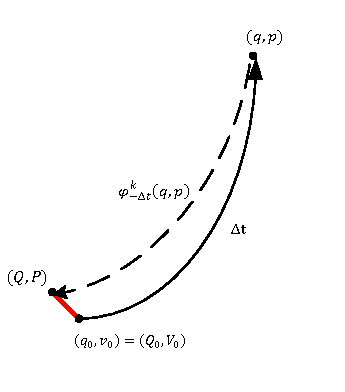
\includegraphics[width=.400\textwidth]{Aldagaialdaketa1}
}
\subfloat[Aldagai berrien integrazioa.]{
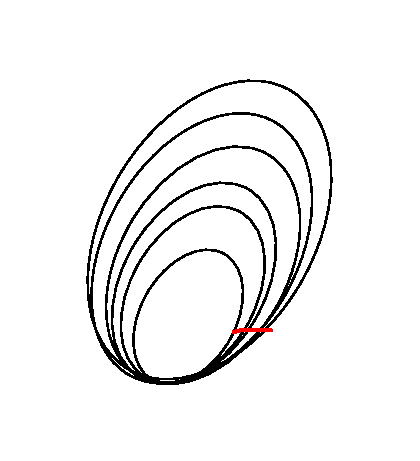
\includegraphics[width=.400\textwidth]{Aldagaialdaketa2}
}
\caption[Atalen hasieraketa.]
        {\small (a)irudian, aldagai aldaketa irudikatu dugu eta (b) irudian, perturbatutako gorputza baten orbitaren integrazioak erakutsi ditugu. Bi irudietan, $(Q,P)$ balioen aldaketa txikiak gorriz nabarmendu ditugu          
        }
\label{fig:Aldg}
\end{figure}   

\subsection*{Integrazioa.}
Aldagai berrien araberako Hamiltondarra honakoa da,
\begin{align}
\begin{split}
&\mathcal{H}(Q,P,t)=H_I (\varphi_{t-t_0}^K(Q,P),t):=G (Q,P,t).
\end{split}
\end{align}
eta hauek dira ekuazio diferentzialak,
\begin{align}
\begin{split}
&\frac{d Q_i}{dt}= +\frac{\partial G}{\partial P_i} (Q,P,t),\\
&\frac{d P_i}{dt}= -\frac{\partial G}{\partial Q_i} (Q,P,t), \ i=1,\dots,d.\\
\end{split}
\end{align}


Hurrengo ataletan, ekuazio diferentzialen konputazioaren zehaztapenak emango ditugu. Lehenik, gorputz bakarraren problema, hau da, alde Kepleriar bakarra duen kasu partikularra aztertuko dugu. Bigarrenik, $N>1$ gorputzen problemarekin, alde kepleriar bat baino gehiago duen kasu orokorra aztertuko dugu. 

\subsubsection{Alde Kepleriar bakarra.}

Satelite baten orbitaren ekuazio diferentzialak, era honetan idatz daitezke,
\begin{align}
\begin{split}
&\frac{d}{dt}\left(\begin{array}{c}
                q  \\
                v  \\
\end{array}\right)
= k(t,q,v)         
+ g(t,q,v), \\
&k(t,q,v)=\left(\begin{array}{c}
                 v \\
                -\frac{\mu}{\|q\|^3} \ q\\
\end{array}\right),
\end{split}
\end{align}
non $q,v \in \mathbb{R}^3$ diren. Azpimarratu nahi dugu, $g(t,q,v)$ perturbazioa ez duela zertan Hamiltondarra izan behar.

Fluxuan oinarritutako aldagai aldaketa aplikatzen badugu,
\begin{equation}
\left(\begin{array}{c}
                q  \\
                v  \\
\end{array}\right)= \varphi_t(Q,V),
\end{equation}

aldagai berriei dagozkien ekuazio diferentzialak era honetan definitzen dira (ikus \ref{erans:B4} eranskinean garapen osoa),
\begin{align}
\label{eq: gEAld}
\frac{d}{dt}\left(\begin{array}{c}
                Q(t)  \\
                V(t)  \\
\end{array}\right) =(\varphi'_t(Q,V))^{-1} \ g.
 \end{align}


\paragraph*{Algoritmoa.}
$(Q,V)$ aldagaien integrazioa, hiru urratsetan egingo dugu:
\begin{enumerate}
\item $\{q,v,aux\} \leftarrow KeplerFlowGen (t,Q,V,mu)$.

Kepler-en fluxua $(q,v)= \varphi_t(Q,V)$ aplikatuko dugu eta fluxuaren kalkulutarako erabilitako tarteko balioak, ~$aux\in \mathbb{R}^{16}$ aldagaian itzuliko ditugu. 

\item $g \leftarrow g(t,q,v)$.

Perturbazioei dagokien ekuazio diferentziala aplikatuko dugu.

\item $KeplerFlowGFcnaux(aux,Q,V,t,g)$.

Lehenik, $\varphi'_t(Q,V))$ modu eraginkorrean kalkulatu behar da. Deribazio automatikoaren teknikaren bidez, Kepler fluxuaren deribatuaren konputazio eraginkorra definitu dugu. 

Ekuazio diferentzialen (\ref{eq: gEAld}) espresioaren konputazioa egingo dugu,   
\begin{align*}
&KeplerFlowGFcnaux(aux,Q,V,t,g)= ( \varphi'_t(Q,V))^{-1} \ g.
\end{align*}

\end{enumerate} 


\subsubsection*{Alde Kepleriar bat baino gehiago.}

Alde Kepleriar bat baino gehiago dugun problemen azterketa egingo dugu. Problemaren alde Kepleriarren kopurua $k$ bada, era honetako ekuazio diferentzialak ditugu,
\begin{equation*}
\frac{d}{dt}\left(\begin{array}{c}
                q  \\
                v  \\
\end{array}\right)=
\left(\begin{array}{c}
                q_1  \\
                v_1  \\
                q_2  \\
                v_2  \\
                \vdots \\
                q_k    \\
                v_k    \\
                w      \\
\end{array}\right)=
\left(\begin{array}{c}
                v_1  \\
                -\mu_1 \ q_1/\|q_1\|^3  \\
                v_2  \\
                -\mu_2 \ q_2/\|q_2\|^3  \\
                \vdots \\
                v_k    \\
                -\mu_k \ q_k/\|q_k\|^3  \\
                0      \\
\end{array}\right)+
g(t,q_1,v_1,\dots, q_k,v_k,w),
\end{equation*} 
non 
\begin{equation*}
g(t,q_1,v_1,\dots, q_k,v_k,w)=
\left(\begin{array}{c}
                g_1(t,q_1,v_1,\dots, q_k,v_k,w)      \\
                g_2 (t,q_1,v_1,\dots, q_k,v_k,w)     \\
                \vdots   \\
                g_k (t,q_1,v_1,\dots, q_k,v_k,w)      \\
                g_{k+1}(t,q_1,v_1,\dots, q_k,v_k,w)    \\
\end{array}\right).
\end{equation*}

Gorputz bakoitzari dagokion aldagai aldaketa lokala da,
\begin{align}
\label{eq:aldfl2}
\begin{split}
\left(\begin{array}{c}
                q_j  \\
                v_j  \\
\end{array}\right)&= \varphi_t^{\mu_j}(Q_j,V_j), \ \ \ j=1,\dots,k, \\
w&=W.
\end{split}
\end{align}

Aldagaia berriekiko ekuazio diferentzialak honakoak dira (ikus \ref{erans:B4} eranskinean garapena),
\begin{equation*}
\frac{d}{dt}
\left(\begin{array}{c}
                Q_1  \\
                V_1  \\
                \vdots \\
                Q_k    \\
                V_k    \\
                W      \\
\end{array}\right)=
\left(\begin{array}{c}
               \varphi_t'^{\ \mu_1}(Q_1,V_1)^{-1} \ g_1 \\ 
               \varphi_t'^{\ \mu_2}(Q_2,V_2)^{-1} \ g_2 \\
               \vdots \\
               \varphi_t'^{\ \mu_k}(Q_k,V_k)^{-1} \ g_k \\
               g_{k+1}
\end{array}\right).
\end{equation*}



\subsection*{Metodo simetrikoa.}

Lehenik, azpimarratu behar dugu aldagai aldaketa lokala izan behar duela eta horretako, integraziorako egoera aldagai berri bat ($\tau$) gehitu behar dugula,
\begin{equation}
(U,\tau).
\end{equation}

Metodoa simetriko izateko integrazio eskema orokorra, \ref{fig:proiekzioa1} eta \ref{fig:proiekzioa2} irudietan laburtu dugu. $u_i$ jatorrizko aldagaiak eta $U_i$ aldagai berriak adierazten duten notazioa erabiliko dugu. Hauek dira, integratzeko emango ditugun urratsak:
\begin{enumerate}
\item \emph{Startfun} funtzioa.

Lehenengo, $u_0$ jatorrizko aldagaien hasierako baliotik abiatuta, aldagai berriei dagokion hasierako balioa finkatuko dugu.
\begin{align*}
u_0 \ \rightarrow \ (U_0,-h/2).
\end{align*}


\item \emph{Urratsa}.

Urratsa integrazio eta proiekzioaren konposaketa da; \ref{fig:proiekzioa2} irudian zehaztapenak eman ditugu. Aldagai aldaketa urrats bakoitzean aplikatzen dugu eta horregatik, integratu ondoren, zenbakizko soluzioaren jatorrizko aldagaietara proiekzioa egiten dugu.  
\begin{align*}
(U_0,-h/2) \ \rightarrow \ (U_1,-h/2).
\end{align*}

Biribiltze errorea txikitzeko, proiekzioa doitasun altuan konputatzea garrantzitsua da. Era honetan, batura konpensatua aplikatzerakoan zifra batzuk irabaziko ditugu. 


\item \emph{Outputfun} funtzioa.

Erabiltzaileak definitutako urratsetarako, $u_n$ jatorrizko aldagaietan zenbakizko soluzioa itzuliko dugu.
\begin{align*}
(U_n,-h/2) \ \rightarrow \ u_n.
\end{align*}


\end{enumerate}



\begin{figure} [h!]
\centerline{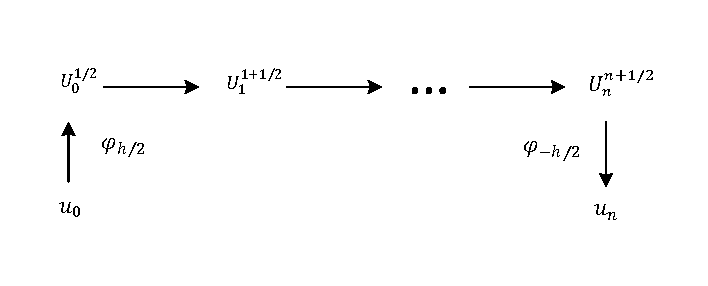
\includegraphics [width=12cm, height=4cm] {proiekzioa1}}
\caption{\small $u_i$ jatorrizko aldagaiak eta $U_i$ aldagai berriak adierazten dute. Lehenengo, $u_0$ jatorrizko aldagaien hasierako baliotik abiatuta, aldagai berriei dagokion hasierako balioa finkatuko dugu $(U_0,-h/2)$. Urrats bakoitza, integrazio eta proiekzioaren konposaketa da eta \ref{fig:proiekzioa2} irudian zehaztu dugu. Erabiltzaileak definitutako urratsetarako, $u_n$ jatorrizko aldagaietann zenbakizko soluzioa itzuliko dugu}
\label{fig:proiekzioa1}
\end{figure} 

\begin{figure} [h!]
\centerline{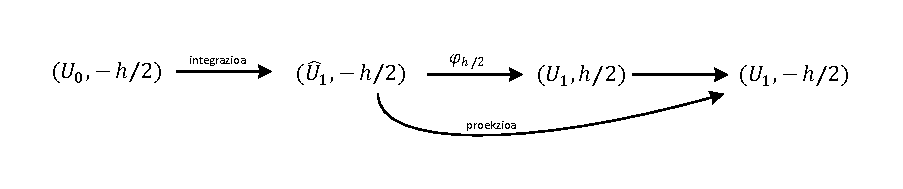
\includegraphics [width=10cm, height=3cm] {proiekzioa2}}
\caption{\small \ref{fig:proiekzioa2} irudiko urrats bakoitzaren zehaztapenak: lehenengo integratzen dugu eta ondoren proiekzioa aplikatzen dugu}
\label{fig:proiekzioa2}
\end{figure} 


Gauss metodoa, neurri batean  Splitting eta konposizio metodoen baliokideak dira. 
\begin{align*}
&\text{Konposizio metodoa} \ \ \Leftrightarrow \ \ \text{Gauss metodoa aldagai aldaketa gabe}.\\
&\text{Splitting metodoa}  \ \ \Leftrightarrow \ \  \text{Gauss metodoa aldagai aldaketarekin}.
\end{align*}

Splitting metodoekiko antzekotasuna azaltzeko, (\ref{eq:stverlet})~\emph{Störmer-Verlet} Splitting metodoarekin konparatuko dugu. \emph{Störmer-Verlet} metodoa, era honetan aplikatzen da: $h/2$ fluxua aplikatu, perturbazioak kalkulatu eta berriz  $h/2$ fluxua aplikatu. Fluxuaren aldagai aldaketarekin, gauza bera egiten ari gara: $h/2$ fluxua aurreratu, perturbazioak kalkulatu (aldagai berrietan eta beraz, hobeto kalkulatzen dugu), $h/2$ fluxua aurreratu. 


\section{Zenbakizko esperimentuak.}


Atal honetan, puntu-finkoaren iterazioan oinarritutako Gauss metodoaren inplementazioa erabili dugu eta eguzki-sistemaren ekuazio diferentzialei, Kepler-en fluxuan oinarritutako aldagai aldaketa aplikatu diegu. $s=6,8,9,16$ ataletako Gauss metodoak exekutatu ditugu eta metodo eraginkorrena aukeratu dugu, ordena altuko beste metodo sinplektikoekin konparatzeko. 


\subsection{Problemak.}


9-planeten problema erabili dugu integrazioetarako. Hasierako balioak \emph{DE-430} efemerideen artikulutik hartu ditugu: planeten masak  (\ref{tab:9bodymas}) taulan laburtu ditugu; hasierako kokapen eta abiadurak (\ref{tab:9bodyhas}) aurki daitezke. Integratzeko, koordenatu heliozentrikoei dagozkien Hamiltondarrean (\ref{eq:nbodyHel}) oinarrituko gara. 

Integrazioaren tartea $(0,10^5)$ egunetakoa izan da. Metodoak integratzeko urrats luzerak $s$-ren proportzionalak aukeratu ditugu:
\begin{align*}
&s=6: \ h=2^{k/4}, \ k=4,\dots,28, \\
&s=8: \ (8/6)h \\
&s=9: \ (9/6)h \\
&s=16: \ (16/6)h \\
\end{align*} 

Zenbakizko esperimentuetarako, aldagai aldaketa planeta guziei aplikatzea erabaki dugu. $9$-planeten probleman, gorputz kopurua txikia denez,  Kepler fluxuaren gainkarga garrantzitsua da eta  barne-planetei bakarrik aplikatzea, eraginkorragoa izan daiteke. Baina, gorputz gehiago kontsideratzen baditugu (esaterako ilargia eta asteroide nagusienak) edo eguzki-sistemaren eredu konplexuagoetan (esaterako erlatibitate efektua gehitzerakoan), perturbazio aldearen konputazioa nagusituko da eta Kepler fluxuaren kalkuluak pisua galduko du. 


\subsection*{Lehen esperimentua.}


Esperimentu honetan, $s=6,8,9,16$ ataletako metodoen eraginkortasun grafikoak irudikatu ditugu. Eraginkortasuna-fcn grafikoak, metodoak problema erreal batean nola jokatuko luke erakusten digu. Eraginkortasun-denborak, ordea, adibide zehatzean zer gertatzen den.

\begin{figure}[h!]
\centering
\begin{tabular}{c c}
\subfloat[Eraginkortasun grafikoa: errorea CPU denborarekiko]
{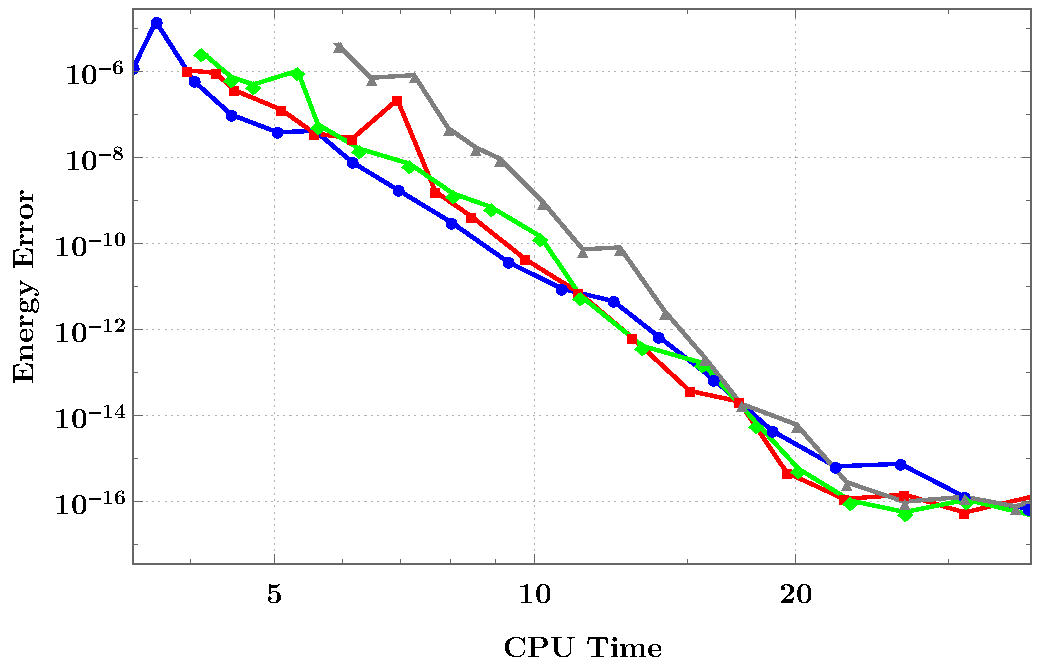
\includegraphics[width=.4\textwidth]{esperimentua811}}
&
\subfloat[Eraginkortasun grafikoa: errorea FCN kopuruarekiko]
{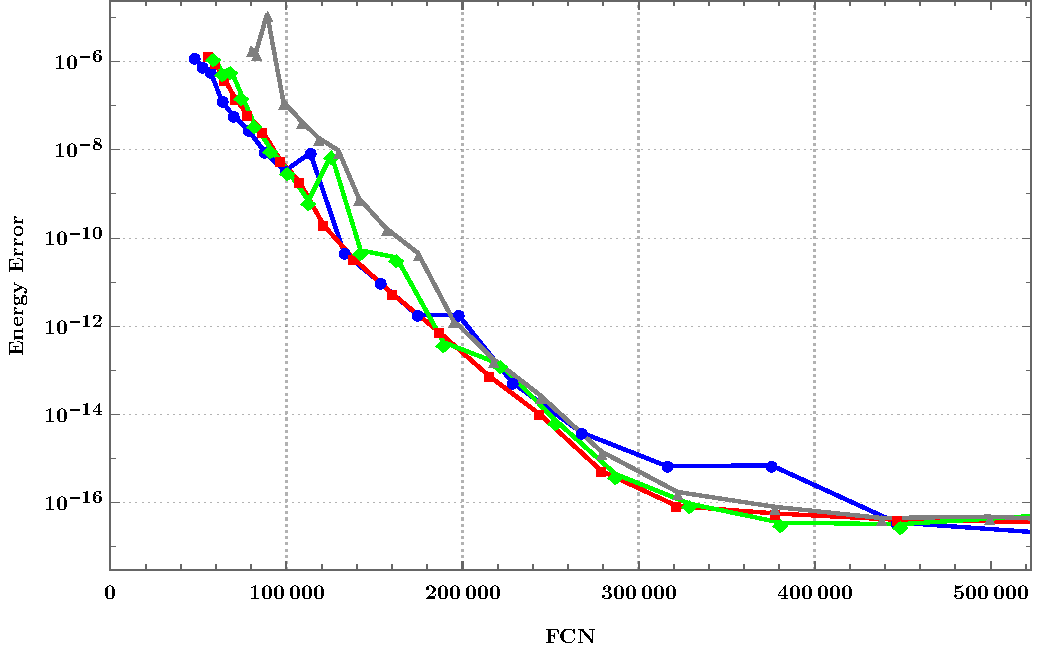
\includegraphics[width=.4\textwidth]{esperimentua812}}
\end{tabular}
\caption{\small 
Eraginkortasun grafikoak irudikatu ditugu: ezkerrean energiaren errore maximoa, CPU denborarekiko; eskuinean ekuazio diferentzialen ebaluazio kopuruarekiko (FCN). Gauss metodoaren lau integrazio konparatu ditugu: $s=6$  urdinez, $s=8$ gorriz, $s=9$ berdez, eta $s=16$ grisez}
\label{fig:esp81}
\end{figure}

\subsection*{Bigarren esperimentua.}


Beste metodo sinplektikoekiko konparaketa.

\begin{figure}[h!]
\centering
\begin{tabular}{c c}
\subfloat[Eraginkortasun grafikoa: errorea CPU denborarekiko]
{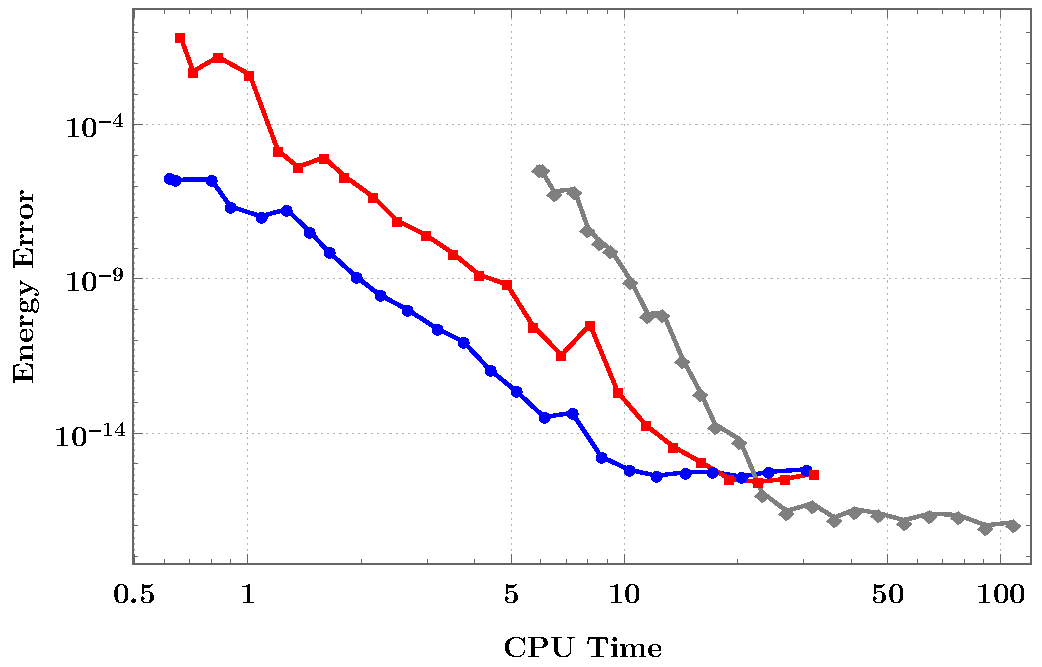
\includegraphics[width=.4\textwidth]{esperimentua821}}
&
\subfloat[Eraginkortasun grafikoa: errorea FCN kopuruarekiko]
{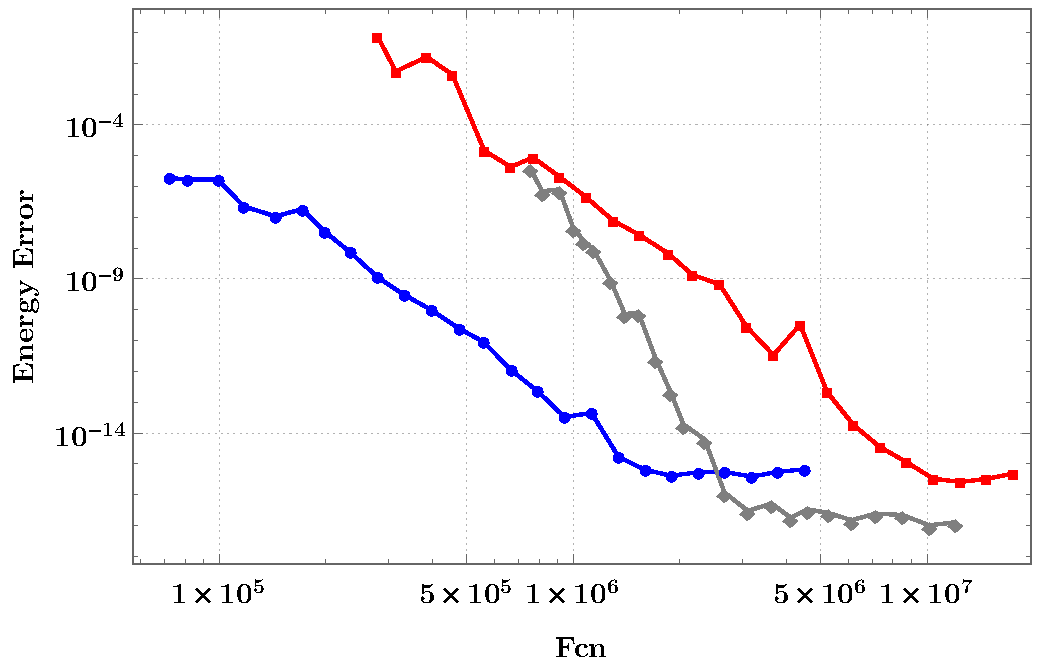
\includegraphics[width=.4\textwidth]{esperimentua822}}
\end{tabular}
\caption{\small 
Eraginkortasun grafikoak irudikatu ditugu: ezkerrean energiaren errore maximoa, CPU denborarekiko; eskuinean ekuazio diferentzialen ebaluazio kopuruarekiko (FCN). Lau integrazio metodo konparatu ditugu: $ABAH1064$  urdinez, $CO1035$ gorriz, $IRK12$ berdez, eta \emph{IRKFLUXU} grisez}
\label{fig:esp82}
\end{figure}

\subsection*{Hirugarren esperimentua.}


Oraingoz era honetan exekutatu ditut esperimentuak. $s=2$ metodoaren bi integrazio: lehena $h=8$ eta bigarrena $h=4$ urratsa luzerarekin. Integrazio tartea $t_{end}=2^{12} h=0, \ h_0=2^4$.


\subsubsection*{Energiaren eboluzioa}

\begin{figure}[h!]
\centering
\begin{tabular}{c c}
\subfloat[Energy errorearen $h=8$.]
{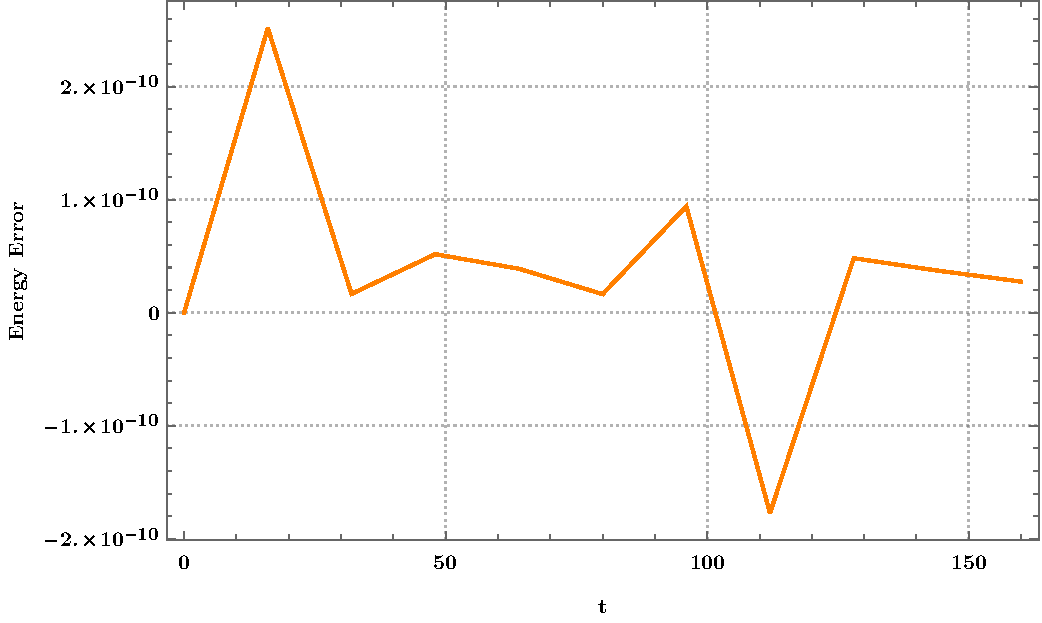
\includegraphics[width=.4\textwidth]{esperimentua831}}
&
\subfloat[Energy errorearen $h=4$.]
{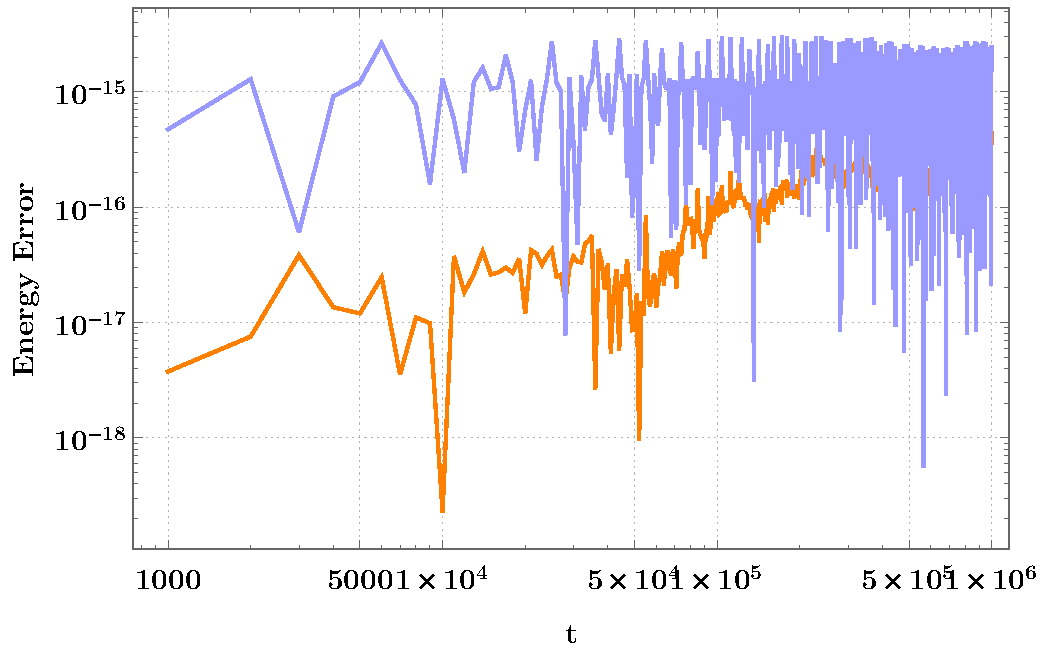
\includegraphics[width=.4\textwidth]{esperimentua832}}
\end{tabular}
\caption{\small }
\label{fig:esp83}
\end{figure}


\subsubsection*{Kokapen errorea}

\begin{figure}[h!]
\centering
\begin{tabular}{c c}
\subfloat[Kokapen errorea.]
{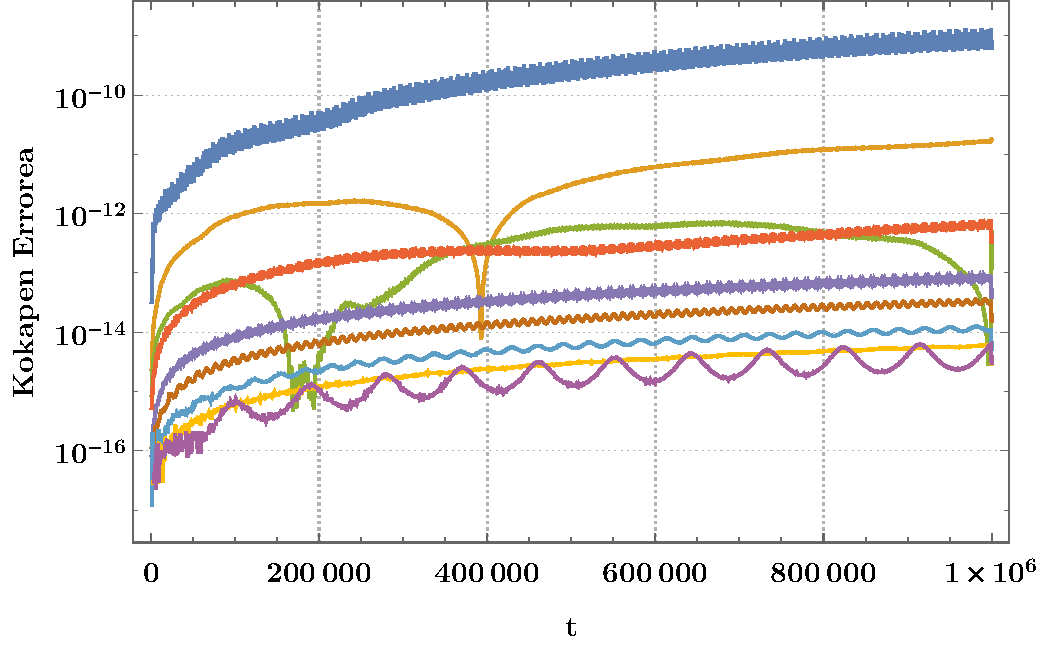
\includegraphics[width=.4\textwidth]{esperimentua841}}
&
\subfloat[Abiadura errorea.]
{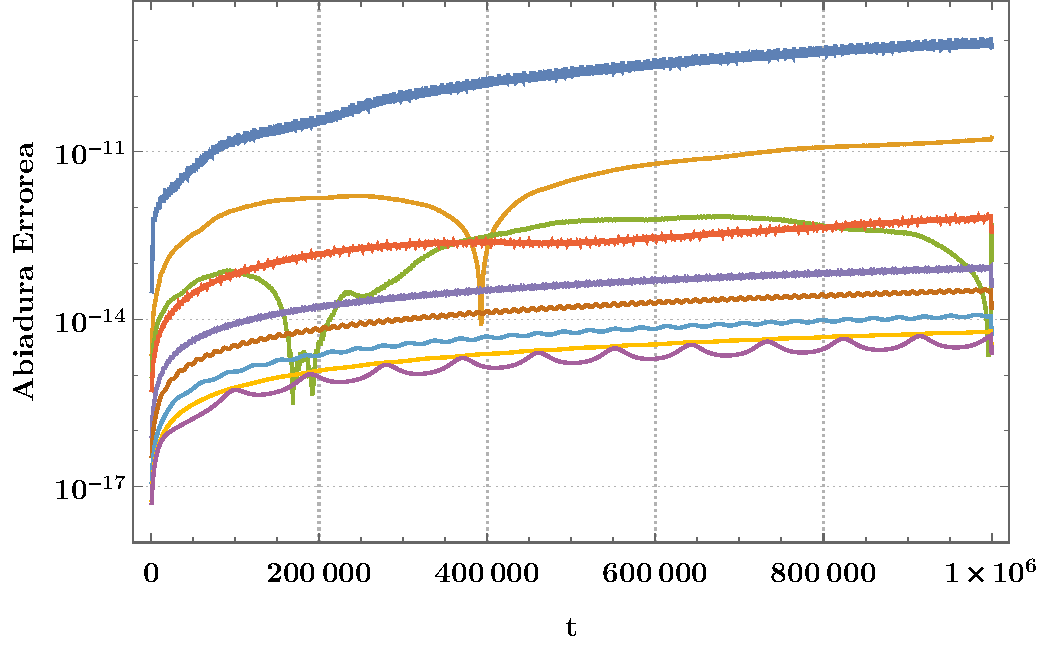
\includegraphics[width=.4\textwidth]{esperimentua842}}
\end{tabular}
\caption{\small }
\label{fig:esp83}
\end{figure}


\subsubsection*{Eszentrikotasun errorea}

Arazoak

\subsubsection*{Semi axis errorea}

Arazoak.


\subsection*{Laugarren esperimentua.}


Biribiltze errorearen azterketa (momentu angeluarra).


\subsection*{Bostgarren esperimentua.}

Paralelizazioa.


\section{Laburpena.}